\section{深入理解X25519}

\subsection{X25519设计理念概述}

Curve25519是Bernstein在2006年构建的蒙哥马利曲线,其中25519表示曲线基于的素数域的特征为$2^{255}-19$.
并在该曲线上构建了仅基于$x$坐标的ECDH密钥协议X25519.
仅利用椭圆曲线点的$x$坐标构建ECDH的想法最初来自于
Victor Miller在1985年发表的奠基性文章"Use of elliptic curves in cryptography"\footnote{
Miller, Victor S. "Use of elliptic curves in cryptography." In Conference on the theory and application of cryptographic techniques, pp. 417-426. Springer, Berlin, Heidelberg, 1985.
\url{https://link.springer.com/content/pdf/10.1007/3-540-39799-X_31.pdf}}.
在仅依赖$x$坐标的ECDH协议中, Alice计算$(a, \mathbf{x}(P))\rightarrow\mathbf{x}(aP)$之后,
将$\mathbf{x}(aP)$传递给Bob, Bob计算$(b, \mathbf{x}(P))\rightarrow \mathbf{x}(bP)$, 
$\mathbf{x}(bP)$传递给Alice, 其中$a$和$b$是Alice和Bob各自生成的临时私钥, $P$为曲线上的一个点.
Alice收到的Bob的消息之后计算$(a, \mathbf{x}(bP)) \rightarrow \mathbf{x}(abP)$,
同样Bob在收到Alice的消息之后,计算$(b, \mathbf{x}(aP))\rightarrow \mathbf{x}(baP)$.
这也是Bernstein的基于Curve25519曲线的X25519的密钥交换协议的基础.
初次接触仅基于$x$坐标系的协议总会感觉有些诡异, 然而考虑到根据$x$坐标和曲线方程,
\textit{基本上}可以完全确定出一个点,例外在于点$P=(x,y)$和$-P=(x,-y)$会有相同的$x$坐标.
通过构建椭圆曲线点群关于逆映射的商群(Quotient Group)$E/\langle - \rangle$,
则在商群的视角下,点的$x$坐标可以唯一表示商群中的元素.
到商群$E/\langle - \rangle$的映射$\mathbf{x}$为
\begin{equation}\label{eq-mapx}
\mathbf{x}: P \rightarrow 
\left\{
\begin{array}{ll}
(x_P : 1)  &\ \text{if}\ P = (x_P : y_P : 1) \\
(1 : 0)      &\ \text{if}\ P = \mathcal{O} = (0: 1: 0)\\ 
\end{array},
\right.
\end{equation}
需要指出的是,写法$\mathbf{x}((X:Y:Z)) = (X:Z)$只有当$Z\neq0$时成立,对于无穷远点$\mathcal{O}$不成立.
对于上述映射$\mathbf{x}$对于点
直观上理解,点$P$和点$-P$在商群中塌缩成同一个元素: $\mathbf{x}(P)=\mathbf{x}(-P)$.
另外点$P, -P$的$k$倍乘运算的结果$kP, k(-P)$在商群$E/\langle - \rangle$中也坍缩成同一个元素: 
$$k(-P) = -kP \implies \mathbf{x}(k(-P)) = \mathbf{x}(-kP)= \mathbf{x}(kP).$$
至此可以理解仅基于$x$坐标可以构建ECDH协议,因为其中仅涉及到群中的倍乘运算.

然而在给定$\mathbf{x}(P)$和$k$的条件下,如何高效计算$\mathbf{x}(kP)$并不显然.
在各种形式表示的椭圆曲线的点群上都可以构建仅基于$x$坐标的运算,但是利用蒙哥马利曲线
上的点群的结构(具体来说是点群中4阶点的存在)配合蒙哥马利阶梯算法更容易完成高效的常量时间实现.
\blue{摘录Bernstein等人在文章``Montgomery curves and the Montgomery ladder"\footnote{
Bernstein, Daniel J., and Tanja Lange. "Montgomery curves and the Montgomery ladder." 
IACR Cryptology ePrint Archive 2017 (2017): 293.
\url{https://eprint.iacr.org/2017/293.pdf}}的表述:
\textit{The Montgomery ladder is much simpler and almost three times faster. The structure of Montgomery curves is important for this simplicity and speed: from the modern Edwards perspective, Montgomery takes advantage of having a point of order 4 on the curve or its twist.}}
这也是Bernstein选择蒙哥马利形式曲线的原因.
在这些原因之外, X25519的设计也考虑到了ECDH的实际部署中的可能遇到的问题
并基于对蒙哥马利曲线的观察进行了巧妙的规避,简化了X25519的实现和应用.

ECDH的实际部署中需要着重考虑的是对接收到的消息的检查.
在典型的ECDH协议中,参与协议的双方都会收到对方发来的临时公钥点,
为了保证安全(例如确保自己的私钥信息不会泄露),需要首先检查收到的点的合法性,
因为如果收到的点是对方刻意构造的点,则对方有可能通过ECDH协议的交互过程窃取私钥信息.
对点的检查通常要验证收到的点不是无穷远点,点的坐标是底层素数域的中的元素并且
确实是椭圆曲线方程上的点.如果没有确认收到的点不是无穷远点,会引发small subgroup攻击;
如果不确认收到的点确实在椭圆曲线上,则会招致invalid-curve攻击,参见
``Guide to elliptic curve cryptography"\footnote{
Hankerson, Darrel, Alfred J. Menezes, and Scott Vanstone. "Guide to elliptic curve cryptography." 
Computing Reviews 46, no. 1 (2005): 13.}中4.3小节.
类似的问题也存在于仅基于$x$坐标的ECDH密钥交换协议当中.
另外仅利用$x$坐标的另一问题在于验证``点在椭圆曲线上"会更困难一些.
检查完整的点只需要把横纵坐标带入方程然后验证返程是否成立即可.
在仅基于$x$坐标的ECDH协议中,
要判定给定的$x$值是否合法等价于判定$x^3+Ax^2+x$是否是二次剩余.
由于域上的平方运算是2-to-1的映射, $x$的所有可能取值大概只有一半的$x$是合法的.
这也是X25519的另一个创新之处:将二次扩域上的椭圆曲线$E(\F_{p^2}), 
\F_{p^2} = \Z_{2^{255}-19}[\sqrt{2}]$的点群纳入考量.
同时考虑两个点群$E(\F_{p})$和$E(\F_{p^2})$,则任意的$x\in\F_p$都可以对应到某个点群上的点,
则前述的需要判定二次剩余来判定$x$是否是合法值的步骤可以省略,
另外由于X25519仅依赖$x$坐标,所以虽然引入了$E(\F_{p^2})$,但X25519所有的运算仍是在域$\F_p$上完成的.
这也是除了仅依赖$x$坐标之外, X25519相比其他的ECDH过程,个人认为最迥异的地方:
为了使所有的$x\in\F_p$都是合法的公钥从而省去繁重的公钥合法性验证,引入了扩域上的椭圆曲线点群.
只要在两个点群上的离散对数问题都是困难的, X25519密钥交换协议就是安全的.

\subsection{深入理解Curve25519与X25519}

蒙哥马利形式的椭圆曲线Curve25519和Curve448被收录在RFC 7748中,
其中Curve448是Mike Hamburg在2015年设计的新曲线,旨在提供224比特的安全性\footnote{
Hamburg, Mike. Ed448-Goldilocks, a new elliptic curve. IACR Cryptology ePrint Archive 2015 (2015): 625.
\url{https://eprint.iacr.org/2015/625.pdf}}.
RFC 7748也同时给出了基于两条椭圆曲线的仅依赖$x$坐标的ECDH密钥交换协议X25519和X448.
本文重点关注Curve25519及相应的密钥交换协议X25519.
Curve25519是定义在有限域$\F_p, p = 2^{255}-19$的蒙哥马利形式椭圆曲线$y^2 = x^3 + 486662x^2 + x$,
其中曲线上点的个数$\#E(\F_p) = 8 \cdot n_1$,也即余因子为8, 并且有\\
\centerline{$n_1=\texttt{0x1000000000000000000000000000000014def9dea2f79cd65812631a5cf5d3ed}$,}


\begin{lstlisting}[language=python, caption=Curve25519的Sage示例, label=lst-curve255619-sage]
sage: fp25519 = FiniteField(2^255-19)
sage: A = fp25519(486662)
sage: B = fp25519(1)
sage: curve25519 = EllipticCurve(fp25519, [0, A, 0, B, 0])
sage: card = curve25519.cardinality()
sage: hex(int(card))
'0x80000000000000000000000000000000a6f7cef517bce6b2c09318d2e7ae9f68L'
sage: n1 = int(card / 8)
sage: hex(n1)
'0x1000000000000000000000000000000014def9dea2f79cd65812631a5cf5d3edL'
sage: curve25519.abelian_group()
Additive abelian group isomorphic to 
Z/57896044618658097711785492504343953926856930875039260848015607506283634007912 
embedded in Abelian group of points on Elliptic Curve defined by 
y^2 = x^3 + 486662*x^2 + x over Finite Field of size 
57896044618658097711785492504343953926634992332820282019728792003956564819949
sage: def print_point(p):
....:     if p.order() == 1:
....:         print "point at infinity"
....:     else:
....:         x, y = p.xy()
....:         print "(%064x,\n %064x)" % (x, y)
....:
sage: G = curve25519.lift_x(9)
sage: print_point(G)
(0000000000000000000000000000000000000000000000000000000000000009,
 5f51e65e475f794b1fe122d388b72eb36dc2b28192839e4dd6163a5d81312c14)
sage: print_point(-G)
(0000000000000000000000000000000000000000000000000000000000000009,
 20ae19a1b8a086b4e01edd2c7748d14c923d4d7e6d7c61b229e9c5a27eced3d9)
sage: P = curve25519.random_point()
sage: while true:
....:     P = n1 * P
....:     if P.order() == 8:
....:         break
....:     P = curve25519.random_point()
....:
sage: print_point(P)
(57119fd0dd4e22d8868e1c58c45c44045bef839c55b1d0b1248c50a3bc959c5f,
 173a6c76c2ba719bce3935ffba04afeadf5bbcb971559722f0efc7bdfb7f9a36)
sage: for i in range(1,9):
....:     p = i * P
....:     print "order = %d" % p.order()
....:     print_point(p)
....:
order = 8
(57119fd0dd4e22d8868e1c58c45c44045bef839c55b1d0b1248c50a3bc959c5f,
 173a6c76c2ba719bce3935ffba04afeadf5bbcb971559722f0efc7bdfb7f9a36)
order = 4
(0000000000000000000000000000000000000000000000000000000000000001,
 141b0b6806563d503de05885280b59109ca5ee38d7b56c9c165db7106377bbd8)
order = 8
(00b8495f16056286fdb1329ceb8d09da6ac49ff1fae35616aeb8413b7c7aebe0,
 46ce3ed6a9617c5ad6b7d3eb19d74ba86cc403d6127fe4b29778eb7c6daf84d3)
order = 2
(0000000000000000000000000000000000000000000000000000000000000000,
 0000000000000000000000000000000000000000000000000000000000000000)
order = 8
(00b8495f16056286fdb1329ceb8d09da6ac49ff1fae35616aeb8413b7c7aebe0,
 3931c129569e83a529482c14e628b457933bfc29ed801b4d6887148392507b1a)
order = 4
(0000000000000000000000000000000000000000000000000000000000000001,
 6be4f497f9a9c2afc21fa77ad7f4a6ef635a11c7284a9363e9a248ef9c884415)
order = 8
(57119fd0dd4e22d8868e1c58c45c44045bef839c55b1d0b1248c50a3bc959c5f,
 68c593893d458e6431c6ca0045fb501520a443468eaa68dd0f103842048065b7)
order = 1
point at infinity
\end{lstlisting}

根据上述Sage示例代码,可以对定义在$\F_p$上的Curve25519椭圆曲线点集有更好的理解.
\code{curve25519.abelian_group()}~的执行结果显示,该点集同构于$\Z_{8n_1}$,
意味着$E(\F_p)$中存在阶为2, 4, 8点.阶为2的点根据曲线方程显然为$(0,0)$.
随后的代码通过随机选取椭圆曲线上的点$P$,并判定$n_1P$的阶是否为8来寻找阶为8的点,
由于点集$E(\F_p)$同构于$\Z_{8n_1}$, 则会有一个8阶的子群,一个$n_1$阶的子群,
8阶子群中有1个1阶点(也即无穷远点), 1个2阶点(也即点$(0,0)$), 2个4阶点,4个8阶点.
每次从点集$E(\F_p)$随机取点$P$,则点$n_1P$的阶为8的概率为1/2,
也即Listing~\ref{lst-curve255619-sage}~中第32至第37行的代码在几次尝试之后即可完成.
有了8阶点之后, Listing~\ref{lst-curve255619-sage}~中第41至45行输出8阶子群中所有点和点的阶.
关于基点$G$, RFC 7748中一开始给出的X25519采用的基点$G$为\\
\centerline{(\texttt{0x9, 0x20ae19a1b8a086b4e01edd2c7748d14c923d4d7e6d7c61b229e9c5a27eced3d9}).}\\
然而在随后的RFC 7748的勘误\footnote{
RFC 7748 Errata. \url{https://www.rfc-editor.org/errata/rfc7748}}
中将基点$G$的具体值修正为\\
\centerline{(\texttt{0x9, 0x5f51e65e475f794b1fe122d388b72eb36dc2b28192839e4dd6163a5d81312c14}).}\\
这是因为, X25519所依赖的椭圆曲线点群运算只涉及点的横坐标,所以X25519涉及的运算只关心横坐标.
然而由于Curve25519与Edwards25519双向有理等价,而Ed25519所依赖的点群运算同时需要横纵坐标,
并且已经有广泛使用的基点的值.
RFC 7748中给出的基点的值,会映射到Edwards25519时会映射成Edwards2519所依赖的基点的负值,
因此有了上述修正,以便在双向有理映射的条件下保持Edwards25519和Curve25519的基点保持一致,
参见Listing~\ref{lst-curve255619-sage}~中第24至第30行.

X25519的设计中为了使得所有的$x\in\F_p$都是合法公钥值引入了二次扩域上的椭圆曲线点群$E(\F_{p^2})$:
$$E(\F_{p^2}) = \{ \mathcal{O} \}  \cup \{ (x,y): y^2 = x^3 + Ax^2 + x,  x, y \in \F_{p^2}, \F_{p^2} = \Z_{2^{255}-19}[\sqrt{2}] \}.$$
定义$E(\F_{p^2})$上的取反操作$-$为: $-\mathcal{O} = \mathcal{O}, -(x,y) = (x,-y)$.
$E(\F_{p^2})$上加法操作$+$定义如下:
\begin{itemize}
\item $\mathcal{O} + \mathcal{O} = \mathcal{O}, \mathcal{O} + (x,y) = (x,y), 
(x,y) + \mathcal{O} = (x,y), (x,y) + (x,-y) = \mathcal{O}$
\item $(x_1, y_1) + (x_2, y_2) = (x_3, y_3)$,
\begin{equation*}
\left\{
\begin{array}{ll}
x_3 & = \lambda^2 - (x_1 + x_2) - A\\
y_3 & = (2x_1 + x_2 + A)\lambda - \lambda^3 - y_1 = \lambda(x_1 - x_3) - y_1\\
\end{array},
\right.
\end{equation*}
其中,
\begin{equation*}
\lambda = 
\left\{
\begin{array}{ll}
(y_2-y_1) / (x_2-x_1),\ \text{if}\ x_1 \neq x_2,\\
(3x_1^2 + 2Ax_1 + 1) / (2y_1),\ \text{if}\ (x_1,y_1) =(x_2,y_2),
\end{array}
\right.
\end{equation*}
\end{itemize}
$E(\F_{p})$显然是$E(\F_{p^2})$中的子群(Subgroup):
$$E(\F_{p}) = \{ \mathcal{O} \} \cup \{ E(\F_{p^2}) \cap \F_p \times \F_p\},$$
根据前述的加法运算规则可知,当$(x_1, y_1), (x_2, y_2) \in  \F_p \times \sqrt{2}\F_{p}$ 时,
$\lambda \in \sqrt{2}\F_p$, 根据运算规则有$(x_3, y_3) \in  \F_p \times \sqrt{2}\F_{p}$.
则有$(x_3, y_3) \in  \F_p \times \sqrt{2}\F_{p}$,所以$E(\F_{p^2})$中的另一个子群为
$$E'(\F_{p}) = \{ \mathcal{O} \} \cup \{ E(\F_{p^2}) \cap \F_p \times \sqrt{2}\F_{p}\}.$$
同时考虑$E(\F_{p})$和$E'(\F_{p})$,则任意的$x\in\F_p, x \neq 0$都对应两个点.
值得注意的是,这两个子群的交集$\{ \mathcal{O}, (0,0) \}$也是$E(\F_{p^2})$的子群.
如前所述,对于所有的$x\in\F_p$,  $E(\F_{p})$和$E'(\F_{p})$中都有2个点的横坐标等于$x$,
例外在于当$x=0$的情况,只有点$(0,0)$的横坐标为零.由于$E(\F_{p})$和$E'(\F_{p})$中都
包含无穷远点$\mathcal{O}$, 则 $\#E(\F_{p})+\#E'(\F_{p}) = 2(p-1) + 2 + 2 = 2p + 2$,
第一次`$+2$'是因为两个集合中均有点$(0,0)$, 第二次`$+2$'是因为两个集合中均有的无穷远点$\mathcal{O}$.
则$\#E'(\F_p) = 2p + 2 - 8n_1 = 4n_2$, 其中
\centerline{$n_2=\texttt{0x1fffffffffffffffffffffffffffffffd6420c42ba10c6534fdb39cb4614581d}$.}
事实上$E'(\F_p)$可以看做是与$E(\F_p)$在$\F_{p^2}$上同构的二次扭曲线(Quadratic Twist)上的点群.
蒙哥马利曲线$E_{A,B}^M$中的两个参数$A, B$中,更重要的是参数$A$,因为$E_{A,B}^M$
的$j$-不变量($j$-invariant)为:
$$j(E_{A,B}^M) = \frac{256(A^2-3)^3}{A^2-4}$$
也即蒙哥马利曲线的$j$-不变量完全由参数$A$定义.
而参数$B$可以被看做是扭曲因子(Twisting Factor): 对于$B' \in \F_p, B' \neq 0$,
则通过符号代换$(x,y)\rightarrow(x,\sqrt{B/B'}y)$有$E_{A,B}^M \cong E_{A,B'}^M$.
当$B/B'$是$\F_p$上的二次剩余时,该同构(Isomorphism)是定义在$\F_p$上的,
否则$E_{A,B'}^M$是$E_{A,B}^M$的二次扭曲线,也即两个曲线在$\F_{p^2}$中是同构的.
对于Curve25519曲线有$B=1$, 根据前述定义$\F_{p^2} = \Z_{p}[\sqrt{2}]$, 
有$B'=2$, 注意到$1/2$不是$\F_p$上的二次剩余,
所以$E_{A,B'}^M$是与$E_{A,B}^M$在$\F_{p^2}$上同构的二次扭曲线,
而前述的$E'(\F_p)$也可以看做是$E_{A,B'}^M$在$\F_{p^2}$上的子群.

同时考虑$E(\F_p)$和$E'(\F_p)$,则对于任意的元素$q\in\F_p$,
都存在点$Q\in E(\F_{p^2})$ ($Q\in E(\F_p) \cup E'(\F_p)$)满足其横坐标值为$q$.
基于此, Bernstein证明了映射$\mathbf{x_0}: E(\F_{p^2}) \rightarrow \F_{p^2}$:
\begin{equation}\label{eq-mapx0}
\left\{
\begin{array}{rr}
 \mathbf{x_0}(\mathcal{O}) &  = 0 \\
\mathbf{x_0}((x,y)) & =  x \\
\end{array}
\right.
\end{equation}
对于任意的整数$n$,和所有的点$Q\in E(\F_{p^2}), \mathbf{x_0}(Q) = q, q \in \F_p$, 
都存在唯一的$s\in\F_p$使得$\mathbf{x_0}(nQ) = s$. 
这个结论也为构建仅依赖$x$坐标的X25519密钥交换协议铺平了道路.
简单陈述下证明过程.对于$q\in\F_p$, 计算$\alpha = q^3 + Aq^2 + q$,
则需要对$\alpha$的值是否为零, 是否是二次剩余以及是否是二次非剩余的情况进行讨论.
\begin{itemize}
\item 
$\alpha = 0$时, 意味着$q=0$, 由于$0^2 = 0$, 因此集合$\{ Q\in E(\F_{p^2}): \mathbf{x_0}(Q) = 0 \} 
= \{ \mathcal{O}, (0,0) \}$, 因此对于任意的$Q\in\{ \mathcal{O}, (0,0)\}$都有$nQ \in \{ \mathcal{O}, (0,0)\}$,
也即$\mathbf{x_0}(nQ) = 0$.
\item 
$\alpha$不为零且为$\F_p$上的二次剩余时,则$q(q^2 + Aq + 1) \neq 0 \implies q\neq 0$.
用$r$表示$\alpha$的平方根,则$\F_{p^2}$上的$\alpha$的平方根只有$\pm r$, 则集合
$\{ Q\in E(\F_{p^2}): \mathbf{x_0}(Q) = q \} = \{ (q,r), (q,-r) \}$.
记$s = \mathbf{x_0}(n(q,r))$, 由于$(q,r)\in E(\F_{p})$, 则有$n(q,r)\in E(\F_p)$, 则$s\in \{1,2,\ldots, p-1\}$.
另外$n(q,-r) = n(-(q,r)) = -(n(q,r)) \implies \mathbf{x_0}(n(q,-r)) = \mathbf{x_0}(n(q,r)) = s$.
因此对于所有的满足$\mathbf{x_0}(Q) = q$的点$Q\in E(\F_{p^2})$, 都有$\mathbf{x_0}(nQ) = s$.
\item
$\alpha$不为零且为$\F_p$上的二次非剩余时, 同样有$q\neq0$. 由于$2$也是$\F_p$上的二次非剩余,
则$\alpha/2$是$\F_p$上的二次剩余,记相应的二次根为$r$, 则$\F_{p^2}$上的二次根只能为$\pm r$,
因此$\{ Q\in E(\F_{p^2}): \mathbf{x_0}(Q) = q \} = \{ (q,r\sqrt{2}), (q,-r\sqrt{2}) \}$.
记$s = \mathbf{x_0}(n(q, r\sqrt{2}))$,
由于$(q,r\sqrt{2})\in E'(\F_{p})$, 则有$n(q,r\sqrt{2})\in E'(\F_p)$, 则$s\in \{1,2,\ldots, p-1\}$.
另外$n(q,-r\sqrt{2}) = n(-(q,r\sqrt{2})) = -(n(q,r\sqrt{2})) \implies 
\mathbf{x_0}(n(q,-r\sqrt{2})) = \mathbf{x_0}(n(q,r\sqrt{2})) = s$.
因此对于所有的满足$\mathbf{x_0}(Q) = q$的点$Q\in E(\F_{p^2})$, 都有$\mathbf{x_0}(nQ) = s$.
\end{itemize}

\begin{figure}[h]
\centering
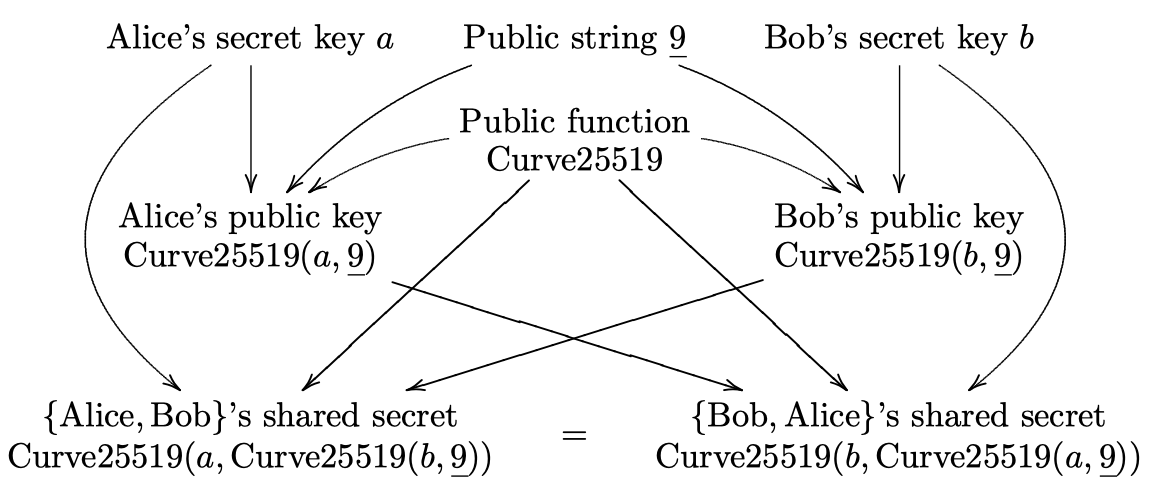
\includegraphics[width=.8\textwidth]{x25519.png}
\caption{X25519密钥交换协议}\label{fig-x25519}
\end{figure}

上述结论证实了在二次扩域视角下,仅依赖$x$坐标也可以进行倍乘运算,
也因此仅依赖二次扩域上的椭圆曲线上点的$x$坐标以及运算可以构建ECDH密钥交换协议,
参见Figure~\ref{fig-x25519}~中展示的Alice和Bob之间的X25519密钥协商过程.
值得注意的是,虽然概念层面上引入了二次扩域但是由于仅依赖$x$坐标,所以倍乘运算还是在$\F_p$上完成的.
Figure~\ref{fig-x25519}~中`Public string \underline{9}'表示X25519的公共参数基点$G$横坐标9的字节数组.
值得提及的是,在X25519和Ed25519的设计文档中,也同时给出了对元素进行编解码的规定.
定义在$\F_p$上的坐标,以小端法编码为字节数组,
也即坐标值$x\in\F_p$与$x[0] + 256  *x[1] + \ldots + 256^{n-1} * x[n-1]$模$p$同余.
从32个字节的数组解码坐标值时,对于X25519协议需要首先将最后一个字节的最高比特位清零,
参见Listing~\ref{lst-x25519-decode}~中第7行,该操作是为了忽略未使用的最高位的比特.
另外,输入参数~\code{bits}~的值为255(对应Curve25519)或者448(对应Curve448).
另外RFC 7748中也明确指出, X25519的协议的实现必须接受非规范(Non-Canonical)的值,
对于X25519而言,非规范的值包括$2^{255}-19$到$2^{255}-1$的所有值.
注意到函数~\code{decodeLittleEndian}~没有对输入参数~\code{u}~做任何限制,
也即32字节的任意值都可以作为Curve25519的公钥$\{\underline{u}, u\in \{0,1,\ldots,2^{256}-1\}\}$.

\begin{lstlisting}[language=python, caption=X25519和X448的编解码, label=lst-x25519-decode]
def decodeLittleEndian(b, bits):
    return sum([ b[i] << 8*i for i in range((bits+7)//8) ])

def decodeUCoordinate(u, bits):
    u_list = [b for b in u]
    # Ignore any unused bits.
    if bits % 8:
        u_list[-1] &= (1 << (bits % 8)) - 1
    return decodeLittleEndian(u_list, bits)

def encodeUCoordinate(u, bits):
    return bytearray([ (u >> 8*i) & 0xff for i in range((bits+7)//8) ])

def decodeScalar25519(k):
    k_list = [b for b in k]
    k_list[0] &= 248  # 1111 1000
    k_list[31] &= 127 # 0111 1111
    k_list[31] |= 64  # 0100 0000
    return decodeLittleEndian(k_list, 255)

def decodeScalar448(k):
    k_list = [b for b in k]
    k_list[0] &= 252
    k_list[55] |= 128
    return decodeLittleEndian(k_list, 448)
\end{lstlisting}

考虑$\mathbf{x}(kP)$中的标量$k$的解析,
参见Listing~\ref{lst-x25519-decode}~中的函数~\code{decodeScalar25519}.
与解码坐标值时类似,解码$k$时将32个字节的数组看成是小端法表示的$k$,
但是按照小端法将字节数组转换成标量$k$之前,
需要将最低3比特清零(第16行), 将最高位清零(第17行), 并将紧邻最高位的比特设置为1 (第19行).
也即X25519的私钥取值空间为$\{\underline{k}: k\in 2^{254} + 8\cdot\{0,1,\ldots,2^{251}-1\}\}$.
将最低3比特清零可以保证私钥值是8的倍数,考虑到Curve25519曲线的余因子为8,
这样可以避免small-subgroup一类的攻击.
将最高位清零,是因为底层素数域的最高位为零,也即公钥的可能取值
将紧邻最高位的比特设置为1,有利于常量时间的蒙哥马利阶梯算法实现\footnote{
StackExchange: When using Curve25519, why does the private key always have a fixed bit at 2\^{}254?
\url{https://crypto.stackexchange.com/questions/11810/when-using-curve25519-why-does-the-private-
key-always-have-a-fixed-bit-at-2254/11818\#11818}}.
值得指出的是,与secp256k1或者secp256r1等曲线的私钥可以在某个区间内连续取值(整数值)不同,
曲线Curve25519上的私钥并不是某个区间内的连续取值,这是为了规避余因子不为1可能引发的安全隐患,
但同时也部分部分影响了曲线的应用方式,尤其是当希望在Ed25519签名算法上实现BIP-32的功能时.
%另外点的倍乘$k\cdot x(P)$可以看做是两个集合到一个集合的映射(非满射):
%$$\{\underline{k}: k\in 2^{254} + 8\cdot\{0,\ldots,2^{251}-1\}\} \times \{\underline{u}, u\in \{0,\ldots,2^{256}-1\}\} \rightarrow \{\underline{u}, u\in \{0,\ldots,2^{256}-1\}\}.$$
%\red{todo: 论证该映射存在的合理性}

至此,介绍了X25519密钥协商协议的设计理念,支撑协议的底层点群结构
以及这些点群结构可以实现仅依赖$x$坐标的倍乘运算的原理, 以及公钥和私钥的取值和编解码转换.
但还未探讨在给定标量$k$和点$P$的横坐标$\mathbf{x}(P)$的条件下如何完成倍乘计算$\mathbf{x}(kP)$.
点的倍乘运算依赖点的加法运算,然而无法直接从$\mathbf{x}(P)$和$\mathbf{x}(Q)$计算$\mathbf{x}(P+Q)$,
因为如前所述$\mathbf{x}(P)$可能对应点$P$也可能对应点$-P$.
$\pm P$与$\pm Q$的点加可能结果为$P+Q, -P+Q, P+(-Q), (-P)+(-Q)$,
可以注意到$\mathbf{x}(P+Q) = \mathbf{x}(-P-Q)$并且$\mathbf{x}(-P+Q) = \mathbf{x}(P-Q)$,
也即$\mathbf{x}(P)$和$\mathbf{x}(Q)$能够完全确定集合$\{ \mathbf{x}(P+Q), \mathbf{x}(P-Q)\}$的值. 
更进一步,集合$\{ \mathbf{x}(P), \mathbf{x}(Q), \mathbf{x}(P+Q), \mathbf{x}(P-Q) \}$中的任意3个元素
可以确定出另外一个元素的值.由此可以定义仅基于$x$坐标的加法运算:
\begin{equation*}
\begin{array}{cc}
\textsf{xADD}: & (\mathbf{x}(P), \mathbf{x}(Q), \mathbf{x}(P-Q)) \rightarrow \mathbf{x}(P+Q) \\
\textsf{xDBL}: & \mathbf{x}(P) \rightarrow \mathbf{x}(2P)
\end{array}
\end{equation*}

考虑点$P=(x_P,y_P), Q = (x_Q, y_Q), P, Q \notin \{\mathcal{O}, (0,0)\}$,
并记$P+Q = (x_{P+Q}, y_{P+Q})$, $P-Q = (x_{P-Q}, y_{P-Q})$, Montgomery发现当$P\neq Q$时,
$x_P, x_Q, x_{P+Q}, x_{P-Q}$之间的关系满足:
\begin{equation}\label{eq-xadd}
x_{P+Q}x_{P-Q}(x_P - x_Q)^2 = (x_Px_Q - 1)^2
\end{equation}
而当$P=Q, P+P = (x_{2P}, y_{2P})$时, $x_P$与$x_{2P}$之间的关系满足:
\begin{equation}\label{eq-xdbl}
4x_{2P}x_P(x_P^2 + Ax_P + 1) = (x_P^2 - 1)^2
\end{equation}
在此处的目标是根据$x_P, x_Q, x_{P-Q}$计算$x_{P+Q}$以及根据$x_P$计算$x_{2P}$.

转换到射影坐标系(Projective Coordinates),并记$\mathbf{x}(P) = (X_P : Z_P)$, 其中$x_P = X_P/Z_P$,
同样有$\mathbf{x}(Q)=(X_Q : Z_Q), \mathbf{x}(P+Q) = (X_{P+Q} : Z_{P+Q}), 
\mathbf{x}(P-Q) = (X_{P-Q} : Z_{P-Q})$. $P, Q \notin \{\mathcal{O}, (0,0)\}$, 则当$P\neq Q$时,
将射影坐标带入方程(\ref{eq-xadd})中有:
\begin{equation*}
\begin{array}{rl}
\frac{X_{P+Q}}{Z_{P+Q}}\frac{X_{P-Q}}{Z_{P-Q}}\left(\frac{X_{P}}{Z_{P}}  - \frac{X_{Q}}{Z_{Q}}\right)^2 = & \left(\frac{X_{P}}{Z_{P}}\frac{X_{Q}}{Z_{Q}} -1\right)^2 \\
\implies \frac{X_{P+Q}}{Z_{P+Q}}\frac{X_{P-Q}}{Z_{P-Q}}\left(\frac{X_PZ_Q - X_QZ_P}{Z_PZ_Q}\right)^2 = & \left(\frac{X_PX_Q - Z_PZ_Q}{Z_PZ_Q}\right)^2 \\
\implies \frac{X_{P+Q}}{Z_{P+Q}}\frac{X_{P-Q}}{Z_{P-Q}}\left(X_PZ_Q - X_QZ_P\right)^2 = & \left(X_PX_Q - Z_PZ_Q\right)^2 \\
\implies X_{P+Q}X_{P-Q}\left(X_PZ_Q - X_QZ_P\right)^2 = & Z_{P+Q}Z_{P-Q}\left(X_PX_Q - Z_PZ_Q\right)^2 \\
\end{array}
\end{equation*}
为保证上式成立,如下指定$X_{P+Q}$和$Z_{P+Q}$的值即可:
\begin{equation*}
\left\{
\begin{array}{ll}
X_{P+Q} & = Z_{P-Q}\left(X_PX_Q - Z_PZ_Q\right)^2\\
Z_{P+Q} & = X_{P-Q}\left(X_PZ_Q - X_QZ_P\right)^2
\end{array},
\right.
\end{equation*}
也等价于
\begin{equation}\label{eq-xadd2}
\left\{
\begin{array}{ll}
X_{P+Q} & = Z_{P-Q}\left[ (X_P-Z_P)(X_Q+Z_Q) + (X_P+Z_P)(X_Q-Z_Q)  \right]^2\\
Z_{P+Q} & = X_{P-Q}\left[ (X_P-Z_P)(X_Q+Z_Q) - (X_P + Z_P)(X_Q-Z_Q)  \right]^2
\end{array},
\right.
\end{equation}
当$P=Q$时, 将射影坐标带入方程(\ref{eq-xdbl})中有:
\begin{equation*}
\begin{array}{rl}
4\frac{X_{2P}}{Z_{2P}}\frac{X_P}{Z_P}\left( \left(\frac{X_P}{Z_P} \right)^2 + A\frac{X_P}{Z_P} + 1\right) = & \left( \left(\frac{X_P}{Z_P}\right)^2 - 1 \right)^2 \\
\implies 
4\frac{X_{2P}}{Z_{2P}}\frac{X_P}{Z_P} \left(\frac{X_P^2 + AX_PZ_P + Z_P^2}{Z_P^2} \right) = & 
\frac{\left(X_P^2 - Z_P^2\right)^2}{Z_P^4}\\
\implies 
4\frac{X_{2P}}{Z_{2P}}(X_PZ_P)\left(X_P^2 + AX_PZ_P + Z_P^2 \right) = & 
\left(X_P^2 - Z_P^2\right)^2\\
\implies 
4X_{2P}(X_PZ_P)\left(X_P^2 + AX_PZ_P + Z_P^2 \right) = & 
Z_{2P}\left(X_P^2 - Z_P^2\right)^2
\end{array}
\end{equation*}
为保证上式成立,如下指定$X_{2P}$和$Z_{2P}$的值即可:
\begin{equation*}
\left\{
\begin{array}{ll}
X_{2P} & = \left(X_P^2 - Z_P^2\right)^2\\
Z_{2P} & = 4(X_PZ_P)\left(X_P^2 + AX_PZ_P + Z_P^2 \right)
\end{array},
\right.
\end{equation*}
也等价于
\begin{equation}\label{eq-xdbl2}
\left\{
\begin{array}{ll}
X_{2P} & = (X_P+Z_P)^2(X_P-Z_P)^2\\
Z_{2P} & = (4X_PZ_P)((X_P-Z_P)^2 + ((A+2)/4)(4X_PZ_P))
\end{array},
\right.
\end{equation}

根据方程(\ref{eq-xadd2})给出的\textsf{xADD}运算过程和方程(\ref{eq-xdbl2})给出的\textsf{xDBL}运算过程
即可完成根据标量$k$和$\mathbf{x}(P)$完成倍乘计算$\mathbf{x}(kP)$.
在继续描述$\mathbf{x}(kP)$的计算过程之前,值得指出的是,
在方程(\ref{eq-xadd2})中没有出现涉及到蒙哥马利曲线的参数$A$和$B$,
而在方程(\ref{eq-xdbl2})中仅涉及到了蒙哥马利曲线的参数$A$,
也即基于$x$坐标的点的运算与参数$B$无关.
前面提到X25519协议为了使所有的$x\in\F_p$都是合法的公钥点,同时考虑了基域上的椭圆曲线的点群$E(\F_p)$
以及二次扩域上的椭圆曲线点群$E'(\F_p)$, 
而$E'(\F_p)$也可以看做是曲线$E_{A,B}^M$的二次扭曲线$E_{A,B'}^M$上的椭圆曲线点群.
由于两个曲线参数中只有$B$不同,因此前述的\textsf{xADD}运算过程和\textsf{xDBL}运算过程
同时适用于两个椭圆曲线点群,而无需区别对待.
另外注意到方程(\ref{eq-xdbl2})中需要完成与$(A+2)/4$的计算,因此在选择曲线参数的时候,
通过选择$A$的值使得$(A+2)/4$的值很小对于加速计算有帮助.
以Curve25519为例, 其中$A = 486662$, 则$(A+2)/4$的值为121665 (十六进制表示形式$\textsf{0x1db41}$).

%由此, 虽然$\xi$并没有直接从$E$中继承运算,但是前述两个点共享同一个横坐标的问题得到解决,
%则$\xi$中可以定义仅依赖于横坐标的运算,并且根据$\xi$和$E$之间的关系,
%该运算规则可以根据$E$中的点的加法运算进行推导.
%而为了支持高速的ECDH密钥协商,要求能够在$\xi$中根据$\mathbf{x}(P)$和标量$k$快速计算$\mathbf{x}(kP)$.
%蒙哥马利阶梯(Montgomery Ladder)算法可以根据$\mathbf{x}(P)$和标量$k$快速计算$\mathbf{x}(kP)$,
%而蒙哥马利曲线的选择可以保证蒙哥马利阶梯算法中的每一步都可以高效执行.

接下来考虑如何利用\textsf{xADD}和\textsf{xDBL}完成点的倍乘运算$\mathbf{x}(kP)$.
首先从Double-and-Add方法说起, 参见Algorithm~\ref{algo-mont-binary}. 
Algorithm~\ref{algo-mont-binary}~可以看做是借助$R_1$完成的Double-and-Add算法的变形.
其中的\textsf{for}循环维持了两个不变量. 
第一个不变量是根据第1, 4, 6行可以观察到的$R_0$和$R_1$之间差值的不变量$R_1-R_0 = P$.
观察Algorithm~\ref{algo-mont-binary}~中对$R_0$的操作, $R_0$在循环开始之前(第1行)被设为$P$,
当$k_i=0$时$R_0\leftarrow 2R_0$ (也即double操作), 
而当$k_i=1$时有$R_0\leftarrow R_0 + R_1 = 2R_0 + P$.
Algorithm~\ref{algo-mont-binary}~实质上借助$R_1$完成了对$R_0$的Double-and-Add操作.
这也引出了Algorithm~\ref{algo-mont-binary}~中的第二个不变量, 在第$i$次迭代中($i$从$\ell-2$
逐次递减到0)有$R_0 = \lfloor k/2^i \rfloor P, R_1 = R_0 + P$, 则当$i = 0$时, 就有$R_0 = kP$,
因此Algorithm~\ref{algo-mont-binary}~正确计算了点的倍乘$kP$.

\begin{algorithm}[h]
\caption{Montgomery's Binary Algorithm}%算法名字
\label{algo-mont-binary}
\LinesNumbered %要求显示行号
\KwIn{$k = \sum_{i=0}^{\ell-1}k_i2^i, k_{\ell - 1} = 1, P \in E_{A,B}(\F_p)$}%输入参数
\KwOut{$kP$}%输出
$(R_0, R_1)  \leftarrow (P, 2P)$\; %\;用于换行
\For{$i = \ell - 2$ down to 0}{
	\eIf{$k_i = 0$}{
		$(R_0, R_1) \leftarrow (2R_0, R_0 + R_1)$\
  	}{
		$(R_0, R_1) \leftarrow (R_0 + R_1, 2R_1)$\
	}
}
\Return $R_0$
\end{algorithm}

基于Algorithm~\ref{algo-mont-binary}~可以发展出计算$\mathbf{x}(kP)$的蒙哥马利阶梯算法(Montgomery Ladder).
用\textsf{xADD}和\textsf{xDBL}替换Algorithm~\ref{algo-mont-binary}~中的点加和点倍乘运算,
同时考虑射影坐标系的表示方法$(X_P:Z_P) = \mathbf{x}(P)$, 可以得到Algorithm~\ref{algo-mont-ladder}.
需要指出的是, 如前所述根据方程(\ref{eq-xadd2})计算两个点的$\textsf{xADD}$时,除了这两个点之外,
还需要这两点的差值. 根据循环不变量,一直有$\textsf{x}_1 - \textsf{x}_0 = P =  (X_P, Z_P)$, 
因此在第4行和第6行, $\textsf{xADD}$的输入参数为$(\textsf{x}_0, \textsf{x}_1, (X_P, Z_P))$.

\begin{algorithm}[h]
\caption{Montgomery's Ladder Algorithm}%算法名字
\label{algo-mont-ladder}
\LinesNumbered %要求显示行号
\KwIn{$k = \sum_{i=0}^{\ell-1}k_i2^i, k_{\ell - 1} = 1, (X_P : Z_P) = \mathbf{x}(P)$}%输入参数
\KwOut{$(X_k, Z_k) = \mathbf{x}(kP),\ \text{if}\ P\notin \{\mathcal{O}, (0,0)\} \ \text{otherwise}\ Z_k = 0$}%输出
$(\textsf{x}_0, \textsf{x}_1)  \leftarrow ((X_P, Z_P), \textsf{xDBL}(X_P, Z_P))$ \; %\;用于换行
\For{$i = \ell - 2$ down to 0}{
	\eIf{$k_i = 0$}{
		$(\textsf{x}_0, \textsf{x}_1) \leftarrow (\textsf{xDBL}(\textsf{x}_0), \textsf{xADD}(\textsf{x}_0, \textsf{x}_1, (X_P, Z_P))$\
  	}{
		$(\textsf{x}_0, \textsf{x}_1) \leftarrow (\textsf{xADD}(\textsf{x}_0, \textsf{x}_1, (X_P, Z_P)), \textsf{xDBL}(\textsf{x}_1))$\
	}
}
\Return $\textsf{x}_0$
\end{algorithm}

在Algorithm~\ref{algo-mont-binary}~和Algorithm~\ref{algo-mont-ladder}~中, $k_i$的值会影响程序的执行流程.
在ECDH协议中, $k$的值通常为协议参与方的私钥, 涉及密钥信息的操作通常希望是常量时间的实现,
也即密钥的取值不应该影响具体的执行流程,否则会泄露关于密钥的信息,从而招致侧信道攻击.
实践中惯用的手法是用加法乘法等运算实现条件交换(Conditional Swap)替换条件判断, 
参见Listing~\ref{lst-curve25519mul}~中函数~\code{cswap}.
Algorithm~\ref{algo-mont-ladder}~用条件交换\textsf{SWAP}改进之后,得到Algorithm~\ref{algo-mont-ladder-const}.
另一处在Algorithm~\ref{algo-mont-ladder}~和Algorithm~\ref{algo-mont-ladder-const}~中展示的尚未解释的
常量时间实现的技术细节也与参数$k$相关.在两个算法输入参数中,都指定了$k_{\ell-1} = 1$,
这是为了使得两个算法中的循环次数与$k$的具体取值无关. 
由于Curve25519定义在255比特的素数域上,因此最高位一直为零,
为了便于常量时间实现, 遵循了同样的常量时间技巧:将次高位比特设置为1,使迭代次数为常数, 
这也是Listing~\ref{lst-x25519-decode}~中执行第18行操作的原因.

\begin{algorithm}[h]
\caption{Constant-Time Montgomery's Ladder Algorithm}%算法名字
\label{algo-mont-ladder-const}
\LinesNumbered %要求显示行号
\KwIn{$k = \sum_{i=0}^{\ell-1}k_i2^i, k_{\ell - 1} = 1, (X_P : Z_P) = \mathbf{x}(P)$}%输入参数
\KwOut{$(X_k, Z_k) = \mathbf{x}(kP),\ \text{if}\ P\notin \{\mathcal{O}, (0,0)\} \ \text{otherwise}\ Z_k = 0$}%输出
$(\textsf{x}_0, \textsf{x}_1)  \leftarrow (\textsf{xDBL}(X_P, Z_P), (X_P, Z_P))$ \; %\;用于换行
\For{$i = \ell - 2$ down to 0}{
	$(\textsf{x}_0, \textsf{x}_1) \leftarrow \textsf{SWAP}(k_{i+1} \oplus k_{i}, (\textsf{x}_0, \textsf{x}_1))$\;
	$(\textsf{x}_0, \textsf{x}_1) \leftarrow (\textsf{xDBL}(\textsf{x}_0), \textsf{xADD}(\textsf{x}_0, \textsf{x}_1, (X_P, Z_P)))$\;
}
$(\textsf{x}_0, \textsf{x}_1) \leftarrow \textsf{SWAP}(k_0, (\textsf{x}_0, \textsf{x}_1))$\;
\Return $\textsf{x}_0$
\end{algorithm}

值得注意的是, Algorithm~\ref{algo-mont-ladder}~和Algorithm~\ref{algo-mont-ladder-const}~在
$P\in\{\mathcal{O}, (0,0)\}$时,无法正确计算$\mathbf{x}(kP)$.
$P\in\{\mathcal{O}, (0,0)\}$时, 返回值为$(X_k, Z_k) = (e, 0)$, 其中$e$可能是零也可能是非零值.
对于仅依赖$x$坐标的ECDH过程,这意味着协议参与方需要执行检查,以确认输入不是$\mathbf{x}(\mathcal{O})$
也不是$\mathbf{x}((0,0))$. Bernstein在构建X25519协议时的另一个贡献是,
通过调整映射$\mathbf{x}$(参见公式(\ref{eq-mapx}))为映射$\mathbf{x_0}$(参见公式(\ref{eq-mapx0})), 
这种对输入参数的检查可以省略. 这意味着蒙哥马利阶梯算法的输入为$(X_P,Z_P)= (x, 1)$, 
其中$x$可以是$\F_p$上的任意的元素, 也即任意的$x\in \F_p$都对应蒙哥马利曲线或者二次扭曲线上的一个点:
$x  = \mathbf{x_0}(P)$. 另外也需要同步修改返回值为$x_k = X_kZ_k^{p-2} \in \F_p$.
这是因为当$Z_k\neq 0$时, 有$x_k = X_k/Z_k$, 而当$Z_k = 0$时, $x_k = 0$, 
两种情形都下都有 $x_k = \mathbf{x_0}(kP)$,另外根据费马小定理有$Z_k^{-1} = Z_k^{p-2}$, 
则蒙哥马利阶梯算法的返回值也统一为$x_k =  X_kZ_k^{p-2} \in \F_p$.

\begin{figure}[h]
\centering
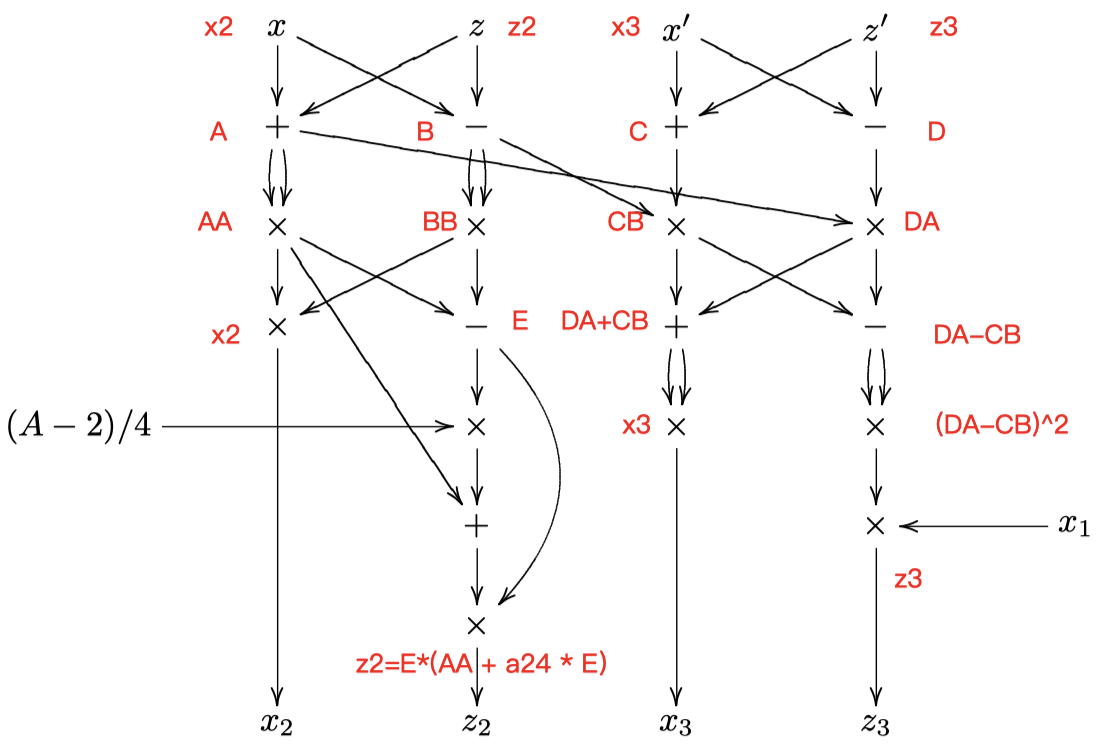
\includegraphics[width=.8\textwidth]{x-coordiniate-add.png}
\caption{X25519密钥交换依赖的点运算}\label{fig-xadd}
\end{figure}

根据方程(\ref{eq-xadd2})和方程(\ref{eq-xdbl2})中展示的$\textsf{xADD}$和$\textsf{xDBL}$中展示的计算过程
以及Algorithm~\ref{algo-mont-ladder-const}~展示的蒙哥马利阶梯算法,可以实现$\mathbf{x}(kP)$, 
参见Listing~\ref{lst-curve25519mul}~中的函数~\code{mul}.
函数~\code{mul}~并不是Algorithm~\ref{algo-mont-ladder-const}~的直接翻译,
而是根据方程(\ref{eq-xadd2})和方程(\ref{eq-xdbl2})中展示的计算过程,
将$\textsf{xADD}$和$\textsf{xDBL}$中的共同操作抽取出来之后的计算过程, 参见Figure~\ref{fig-xadd}.

\begin{lstlisting}[language=python, caption = Curve25519和Curve448上的乘法运算, label=lst-curve25519mul]
# Finite field with p
def FiniteField(p):
    class Fp:
        def __init__(self, val: int):
            assert isinstance(val, int)
            self.val = val
        def __add__(self, other):
            return Fp((self.val + other.val) % Fp.p)
        def __sub__(self, other):
            return Fp((self.val - other.val) % Fp.p)
        def __mul__(self, other):
            return Fp((self.val * other.val) % Fp.p)
        def __rmul__(self, n):
            return Fp((self.val * n) % Fp.p)
        def __pow__(self, e):
            return Fp(pow(self.val, e, Fp.p))
        def __repr__(self):
            return hex(self.val)
        def __int__(self):
            return int(self.val)
    Fp.p = p
    return Fp

def cswap(swap, x_2, x_3):
    "Conditional swap in constant time."
    dummy = swap * (x_2 - x_3)
    x_2 = x_2 - dummy
    x_3 = x_3 + dummy
    return x_2, x_3

def mul(k: int, u: int, bits: int, p: int, a24: int):
    Fp = FiniteField(p)
    x_1 = Fp(u)
    x_2 = Fp(1)
    z_2 = Fp(0)
    x_3 = Fp(u)
    z_3 = Fp(1)
    swap = 0

    for t in range(bits-1, -1, -1):
        k_t = (k >> t) & 1
        swap ^= k_t
        (x_2, x_3) = cswap(swap, x_2, x_3)
        (z_2, z_3) = cswap(swap, z_2, z_3)
        swap = k_t

        A = x_2 + z_2
        AA = A**2
        B = x_2 - z_2
        BB = B**2
        E = AA - BB
        C = x_3 + z_3
        D = x_3 - z_3
        DA = D * A
        CB = C * B
        x_3 = (DA + CB)**2
        z_3 = x_1 * (DA - CB)**2
        x_2 = AA * BB
        z_2 = E * (AA + a24 * E)

    x_2, x_3 = cswap(swap, x_2, x_3)
    z_2, z_3 = cswap(swap, z_2, z_3)
    res = x_2 * (z_2**(p - 2))
    return res
\end{lstlisting}

有了$\mathbf{x}(kP)$的计算方法,则可以实现X25519密钥交换协议, 
参见Listing~\ref{lst-x25519x448}~中的函数~\code{x25519}.
函数~\code{x25519}~根据随机数\textsf{k} (在ECDH协议中是某个参与方的私钥)和
接收到的公钥点\textsf{u}执行点的倍乘运算$\textsf{k}\cdot \textsf{u}$.
基于~\code{x25519}~容易实现X25519密钥交换协议.

\begin{lstlisting}[language=python, caption = X25519与X448的Python示例, label=lst-x25519x448]
def x25519(k: bytes, u: bytes):
    # Curve25519 for the ~128-bit security level.
    # Computes u := k * u where k is the scalar and u is the u-coordinate.
    bits = 255
    k = decodeScalar25519(k)
    u = decodeUCoordinate(u, bits)
    p = 2**255 - 19
    a24 = 121665
    res = mul(k, u, bits, p, a24)
    return encodeUCoordinate(int(res), bits)

def x448(k: bytes, u: bytes):
    # Curve448 for the ~224-bit security level.
    bits = 448
    k = decodeScalar448(k)
    u = decodeUCoordinate(u, bits)
    p = 2**448 - 2**224 - 1
    a24 = 39081
    res = mul(k, u, bits, p, a24)
    return encodeUCoordinate(int(res), bits)
\end{lstlisting}

\subsection{Tendermint中的X25519}

点对点(Peer-to-Peer)通信是区块链技术的典型特征,
以Bitcoin, Ethereum为代表的主流公链中的点对点通信都是明文通信,
交易的全网广播过程会因为明文通信的原因被观测到,
由此可以定位交易的发起方,导致交易隐私的泄露.
也因此改进点对点通信的安全性也是区块链技术演进中的一个技术方向.
典型的改进策略包括调整交易广播过程的??协议,也包括将P2P的明文通信升级为加密通信.

一个区块链项目从架构层面可以分为3个功能层,最底层的是P2P网络通信,
中间的共识协议层以及上层的与具体业务逻辑相关的应用层.
开发区块链项目是困难的, 尤其是涉及到P2P网络通信与共识协议实现.
为了简化区块链项目的开发,出现了Tendermint Core/Cosmos SDK以及Polkadot/Substrate等
致力于为区块链开发提供开发框架的项目.
其中Tendermint Core项目致力于成为构建区块链项目的基础平台,其中实现了Tendermint共识协议以及
完成共识协议所需要的P2P网络通信功能, 而Cosmos SDK项目则为上层应用的开发提供了
一些通用的模块,例如账户模型所需的账户模块, PoS机制所需要的质押等模块.
本文关注Tendermint Core项目中的P2P网络通信层.
Tendermint Core项目中实现了加密通信的P2P协议,
根据白皮书描述该加密通信协议是基于Station-to-Station协议构建的,
具体的密钥协商过程参见Figure~\ref{fig-tendermint-handshake},
图片截取自Cas Cremers和Dennis Jackson的论文\footnote{
}. 虽然X25519和Curve25519在设计时已经尽可能多的考虑应用时的安全陷阱,
然而Cremers和Jackson指出了Tendermint Core中密钥协商过程中存在的安全隐患.
值得注意的是另外一组研究人员也独立发现了Tendermint Core项目中握手协议存在的安全问题\footnote{
}.

\begin{figure}[h]
\centering
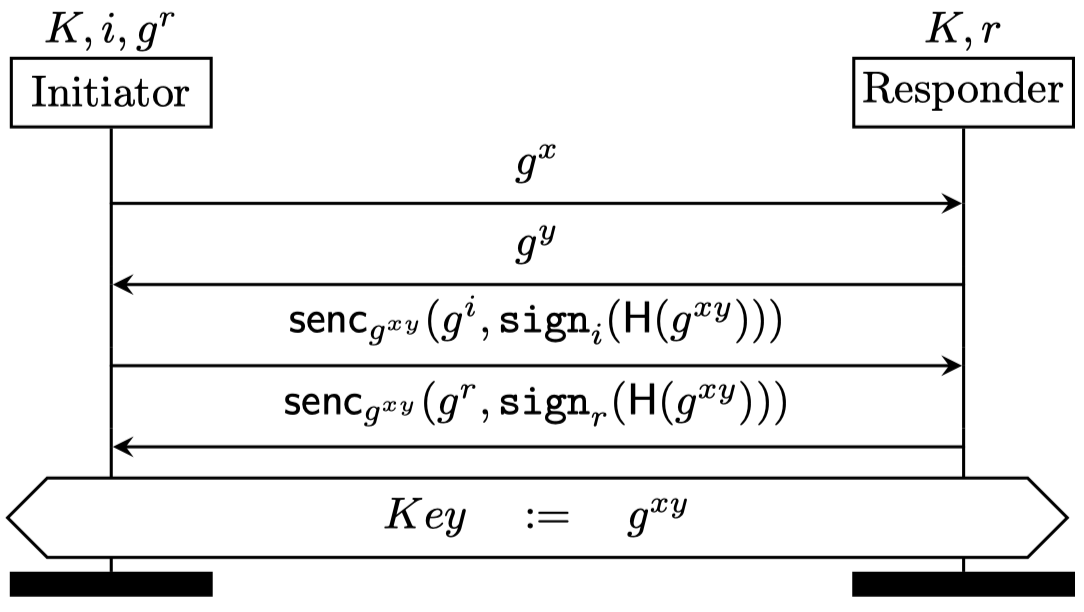
\includegraphics[width=.6\textwidth]{tendermint-handshake.png}
\caption{Tendermint Core中的密钥协商\label{fig-tendermint-handshake}}
\end{figure}